% \textbf{Title: Integral Calculus 3}

The graph of \(f(x)\) is given.

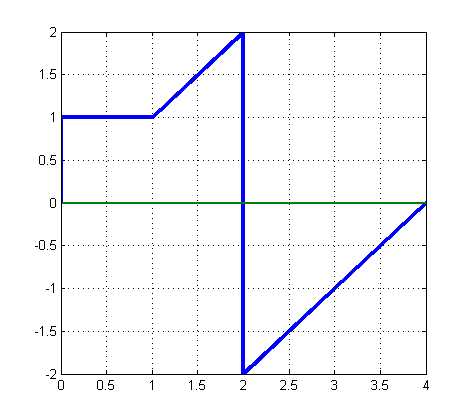
\includegraphics[width=1.71005in,height=1.52489in]{../../Images/IntegralCalculusQ1234.png}

How should \(a\) and \(b\) be chosen to minimise \( \int_a^b f ( x ) \ dx \)?\\


a. \( ( a,\ b ) = ( 0,\ 4 )\)

b. \( ( a,\ b ) = ( 1,\ 3 ) \)

c. \( ( a,\ b ) = (0,\ 2) \)

*d. \( ( a,\ b ) = (2,\ 4) \)

e. I do not know.\\
